%% Semantic Assistants Documentation
%% 
%% This file is part of the Semantic Assistants architecture.
%%
%% Copyright (C) 2009, 2010, 2011 Semantic Software Lab, http://www.semanticsoftware.info
%%
%% The Semantic Assistants architecture is free software: you can
%% redistribute and/or modify it under the terms of the GNU Affero General
%% Public License as published by the Free Software Foundation, either
%% version 3 of the License, or (at your option) any later version.
%% 
%% This program is distributed in the hope that it will be useful,
%% but WITHOUT ANY WARRANTY; without even the implied warranty of
%% MERCHANTABILITY or FITNESS FOR A PARTICULAR PURPOSE.  See the
%% GNU Affero General Public License for more details.
%% 
%% You should have received a copy of the GNU Affero General Public License
%% along with this program.  If not, see <http://www.gnu.org/licenses/>.
%%

\chapter{NLP Service Integration}
\label{chap:services}
In this chapter, we provide additional information for NLP service developers. 

\section{General Process for NLP Service Deployment}
The \sa architecture emphasizes a \emph{separation of concerns}: NLP
pipelines are developed by analysts trained in language technology
(e.g., a certified GATE Text Analyst). The role of the \emph{system
  integrator} is to publish an existing NLP pipeline as a Web
service, published by the \sa server. Two steps are required:
\begin{enumerate}
\item Develop the NLP pipeline as usual, and save it in the default
  \texttt{Resources/GatePipelines} directory (using either the GATE
  Developer \emph{Export for Teamware} option, or the ant packager
  task). Alternatively, you can deploy the pipeline in a custom
  location, which you then define in the \texttt{LocalProperties.xml}
  file (see Section~\ref{sec:props} for details).
\item Create a \emph{service description} in OWL format. The service
  description defines what the optional and required input parameters to the  
  service are, and what results are provided by the service (e.g.,
  document annotations or a result file in any format). The details
  of the \sa service description are defined below.
\end{enumerate}
After deploying the new NLP pipeline together with its OWL service
description, the \sa server needs to be restarted. Clients will
automatically discover any new services deployed in the architecture.

\section{Service Descriptions}\label{sec:owl}
NLP services are described with metadata in OWL format. The ontology
format provides for expressive service description that captures
users, their language capabilities, tools, services, and result
formats. This allows connected clients to \emph{recommend} services
that are suitable for the current user, task, and output capabilities
(e.g., a cell phone has quite different output capabilities from a
netbook or desktop system). 


\subsection{Context and Service Representations}
\label{sec:contextservice}
Clients can request a list of available language services from the
server. Rather than simply returning all available services (which
could be a long list), we want to be able to \emph{recommend} possibly
useful NLP services to the user, based on her context.  In other
words, services that of no use are omitted, e.g., because of language
reasons or missing capabilities of the currently used client.  As a
first, minimal representation of the user's context, we enable a
client to communicate the languages that its user knows, as well as
the language of the document or documents in question. This
representation is recorded in Table~\ref{tab:context}.

\begin{table}[htb]
 \centering\small\sffamily
 \begin{tabular}{p{0.25\textwidth}@{\hspace*{4mm}}p{0.45\textwidth}@{\hspace*{4mm}}p{0.15\textwidth}}
 \toprule
 \textbf{Field} & \textbf{Meaning} & \textbf{Example} \\
 \midrule
 User languages& The languages the user knows& $<$en,de,fr$>$ \\
 Document language&The language of the current document &en \\
 \bottomrule
\end{tabular}
 \caption{Minimal representation of the user context}
 \label{tab:context}
\end{table}

For the client, the point of requesting a list of available language
services is to know which language services exist, and how it can
invoke them. Thus, each description sent by the server contains the
name of the language service it represents, so that the client can
identify it. Secondly, services might contain user-configurable
parameters, so the returned service description also contain a list of
parameter representations. Finally, for practical reasons, the
description holds a short, plain text description to make it clearer
what the language service achieves (examples can be seen in
Figure~\ref{fig:oolist}). Together, this gives us the NLP service
representations shown in Table~\ref{tab:service}

\begin{table}[htb]
 \centering\small\sffamily
 \begin{tabular}{p{0.15\textwidth}@{\hspace*{4mm}}p{0.40\textwidth}@{\hspace*{4mm}}p{0.3\textwidth}}
   \toprule
   \textbf{Field} & \textbf{Meaning} & \textbf{Example} \\
   \midrule
   Service & The name of the language & \emph{Single-document}\\ 
   name & service & \emph{summarizer} \\ 

   & & \\

   Service & Short description of what the & \emph{Creates a summary
     of} \\
   description & service achieves  & \emph{a single document} \\

   & & \\

   Parameter list & List of descriptions illustrated in
   Table~\ref{tab:param} & See Table~\ref{tab:param} \\
   \bottomrule
\end{tabular}
 \caption{Representation of an NLP service}
 \label{tab:service}
\end{table}


While service name and service description are simple strings, the
parameter list needs further clarification. This parameter
representation holds the parameter's name, its data type, and the
information whether the parameter is mandatory or
optional. Table~\ref{tab:param} shows its data fields in detail. In
addition to the mentioned fields, we added a \emph{Parameter value}
field to be written by the client, which it can use to announce
parameter values for a subsequent NLP service invocation. To increase
the usability, we added a \emph{Label} and a \emph{Description} field
that allows a system integrator to add some explaining words to the
parameter representation that are, e.g., helpful for user interface
integration.  The same holds for the \emph{Default Value} field, which
can be used to give the user an idea of what sensible parameter values
are.

% There is one more requirement related to the control of language
% services, and thus parameters. This requirement is Requirement~\#7.3,
% concerning the correct assignment of values.

\begin{table}[htb]
 \centering\small\sffamily
 \begin{tabular}{p{0.2\textwidth}@{\hspace*{4mm}}p{0.50\textwidth}@{\hspace*{4mm}}p{0.2\textwidth}}
   \toprule
   \textbf{Field} & \textbf{Meaning} & \textbf{Example} \\
   \midrule
   Parameter name & The (codified) name of the parameter &
   \emph{outputFormat} \\

   & & \\

   Parameter type & The data type of the parameter & \emph{string} \\

   & & \\

   Optional & Is the parameter optional or mandatory?  & \emph{no} \\

   & & \\

   Parameter value & The value the parameter should take for the
   following invocation. Field to be written by the client. &
   \emph{mediawiki} \\

   & & \\

   Parameter & A short description of the meaning of the & \emph{Use ``mediawiki''} \\
   description & parameter, or advice on its usage & \emph{ or ``html''} \\

   & & \\

   Label & A more expressive name suitable for display in user
   interfaces & \emph{Output format} \\

   & & \\

   Default value & A suitable standard value for the parameter & \emph{html} \\

   \bottomrule
\end{tabular}
 \caption{Representation of a parameter for an NLP service}
 \label{tab:param}
\end{table}

\subsection{The \sa Ontology}
In this section, we provide details on the design of the ontology
used for NLP service descriptions in the \sa architecture.

\subsubsection{The \sa Upper Ontology}
The \sa upper ontology contains five core concepts to model the
relationships between users, their tasks, the artifacts involved and
their format and language. Figure~\ref{fig:centralFive} shows these
five concepts and Table~\ref{tab:top5} provides some descriptions and
examples.

\begin{figure}
  \centering
  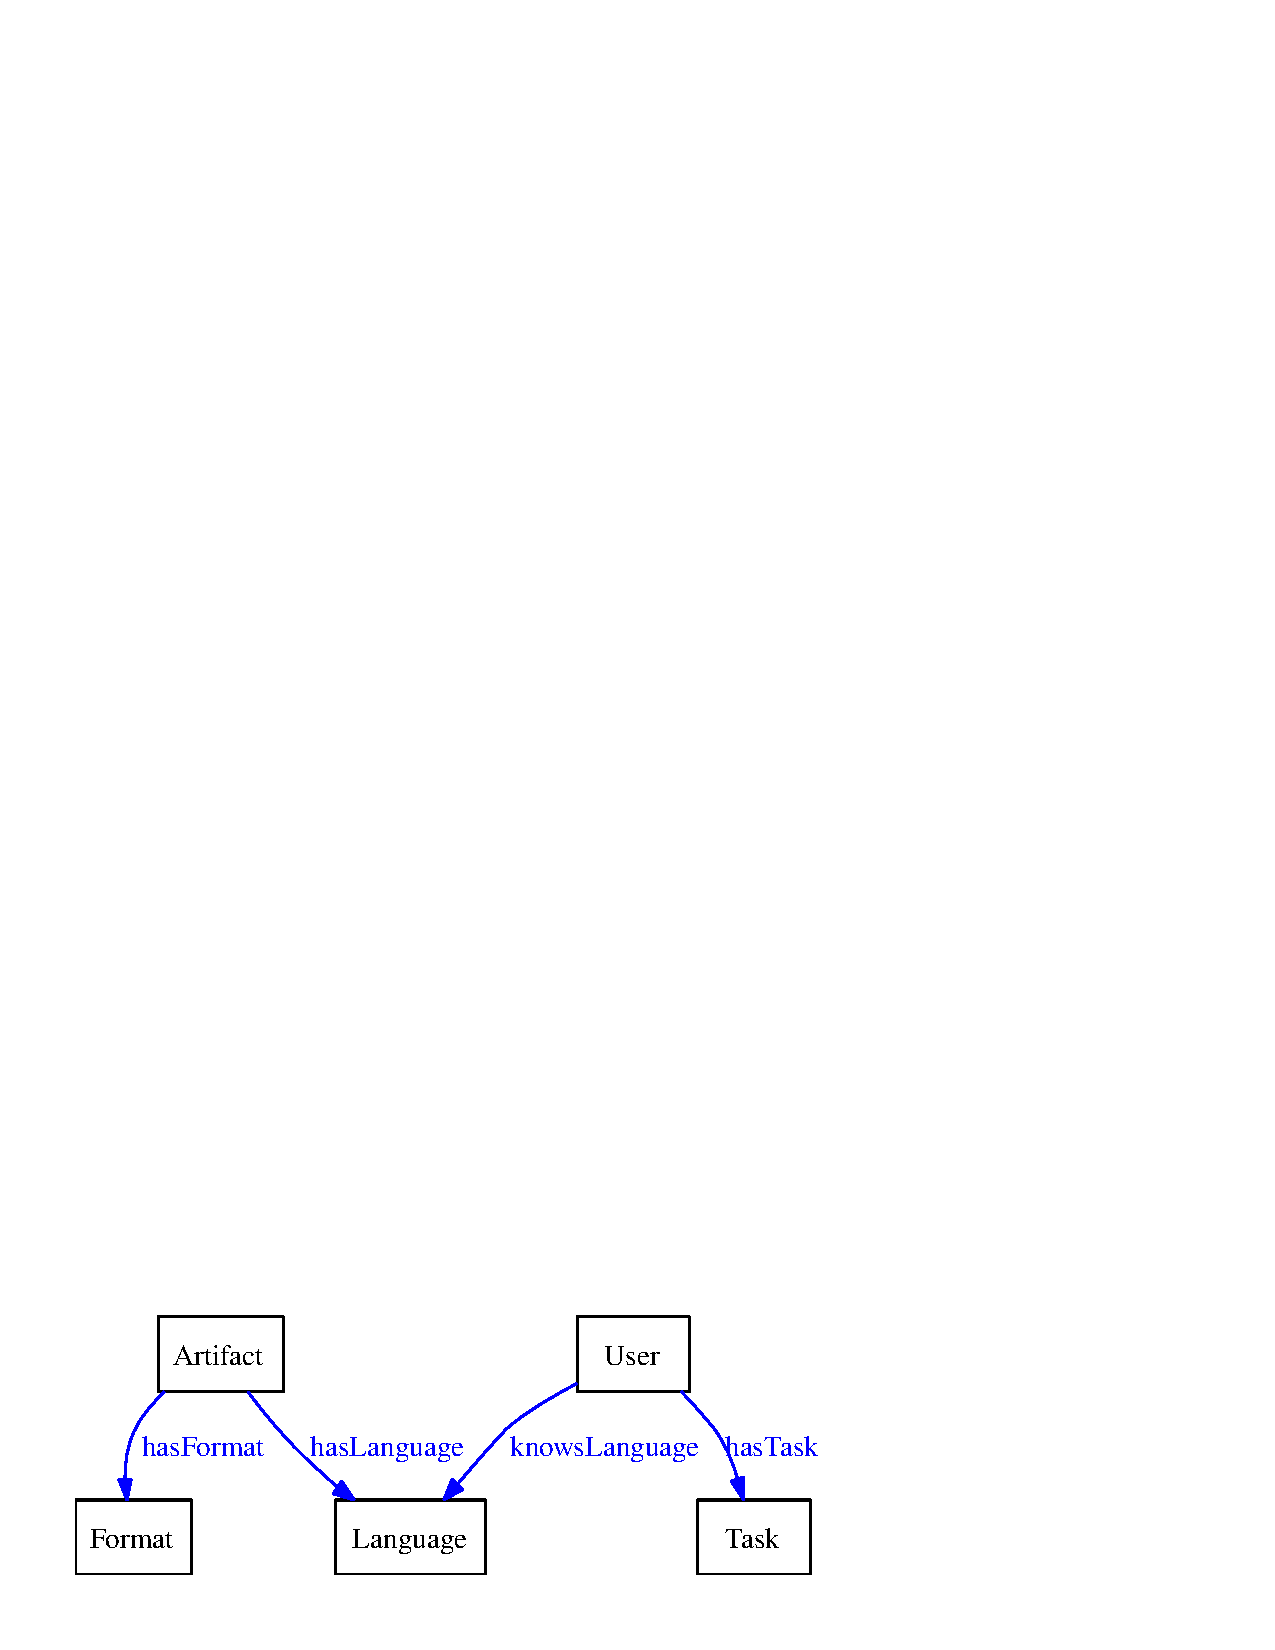
\includegraphics[width=0.5\textwidth]{pictures/centralfive.pdf}
  \caption{The five central concepts of the common upper ontology}
  \label{fig:centralFive}
\end{figure}


\begin{table}[htb]
\centering\small\sffamily
\begin{tabular}{p{0.13\textwidth}@{\hspace*{4mm}}p{0.55\textwidth}@{\hspace*{4mm}}p{0.22\textwidth}}
  \toprule
  \textbf{Concept}&\textbf{Description} &\textbf{Example/sub-concept} \\
  \midrule
  Artifact &The artifact is the central parent concept for all
    kinds of objects like documents, source files, compiled files,
    programs, NLP services, parameters, and annotations. Each field of
    application will most likely introduce its own artifacts.&
    Document, Tool, Parameter\\

   & & \\
  
  Format &Every artifact must have a format. For our language
    service infrastructure, it is important to know what formats the
    input and output of a service have in order to handle them
    correctly. &PDF, HTML\\

   & & \\
  
  User & In order to respond to a user's context, we also have to
    have some knowledge on the user himself. Which 
    languages does he know? What is he working on? & EnglishLearner\\

   & & \\
  
   Language & Languages are orthogonal to formats. Just as it is
   important to know if a file is binary or text, it is important to
   know if it is a Java source file or a manual written in HTML, or
   an article written in Spanish. NLP services are often language
   specific.& English, French, Java\\

   & & \\
  
   Task & Tasks further connect users and services. A task expresses
   a user's goal. If we know that goal, and we know what each of our
   offered services are good for, we can  match the two pieces of
   information and, ideally, provide the user with services that are
   useful to him. & TranslationTask\\
   \bottomrule
\end{tabular}
\caption{The five central concepts of the upper ontology}
\label{tab:top5}
\end{table}

Note that, while artifacts must have a format, they are not required
to have a language. Format information helps us to differentiate
between various kinds of artifacts, e.g., it enables us to tell a GATE
annotation from an executable program. We consider this kind of
information essential and relatively easy to provide -- even if there
is no obvious format, or the format is uncertain, we can most likely
still rely on generic formats like ``plain text file'' or ``binary
file''. On the other hand, it is not always intuitive to give a
language for a given artifact. E.g., we would hesitate to say that a
GATE annotation specifying a part of speech has a certain language.
Likewise, it is not very intuitive to say that a runtime parameter has
a language. Due to these difficulties, we leave the language as an
optional attribute for artifacts.

\paragraph{More Concrete Artifacts.} \emph{Tools}, like an NLP tool,
are a subconcept of \emph{artifacts}. A tool possibly processes
artifacts as input and can produce artifacts as output. These are
modeled with the \emph{consumesInput} and \emph{producesOutput}
relations in our ontology. Moreover, we mentioned parameters that a
tool can have, which is modeled by the \emph{hasParameter}
relation. For our domain, \emph{documents} are of great importance, in
particular natural language documents. These documents all have
languages (English, French, Java, etc.), modeled by the
\emph{hasLanguage} relation. As natural language documents are very
common and important, we introduce a sub-concept of \emph{Document}
called \emph{NaturalLanguageDocument}, which has a
\emph{hasNaturalLanguage} property.

In order to work with documents, they often must somehow be identified
and retrieved. In fact, the \sa server must be able to pull documents
for analysis from the Internet.  Thus, when we model such an input
document in our ontology, we must have a way to specify its URI
(Uniform Resource Identifier) by which we can address it. As not only
documents, but also other artifacts like Web services have to be
uniquely identified and addressed, we introduce \emph{hasIdentifier}
as an optional property for artifacts.  We define
\emph{IdentifiableArtifact} as a class whose members are artifacts and
have this property. In practice, the identifier can, and often will,
be a URI, but it does not have to be. For example, if we have a set of
elements with unique names, a simple string can be enough. With
\emph{hasIdentifier}, we provide an important property on the highest
level, while leaving the exact semantics to the concrete ontologies
and the applications that use them.

\paragraph{Output Modelling.} We introduced one more concept that is
not as obvious as the concepts introduced so far. Suppose there is an
NLP system that can, among others, output XML and OWL files. We would
model artifacts representing these file types, and create the
according \emph{producesOutput} relation pairs. However, which one of
the output variants is produced most likely depends on the way the
NLP system is invoked. Therefore, we have to somewhere store the
information, under which \emph{circumstances} a certain output is
produced. We could store it directly with the individual representing
the output. However, we feel that this information concerns more the
relationship between the system and the output, not the output
itself. Thus, we introduced a concept called \emph{IOArtifact} where
information on input and output relationships can be stored. We will
see a more concrete use of this concept in the following section, when
we concretize the upper ontology. By means of an
\emph{isActualArtifact} relation, we have \emph{IOArtifact}
individuals ``point'' to \emph{Artifact} individuals. They can be seen
as a proxy for artifacts.

We can see the artifact class, its sub-classes, and important
relations between these classes in Figure~\ref{fig:artifact}. A
textual overview is given in Table~\ref{tab:artifact}.
 
\begin{figure*}[htb]
  \centering
  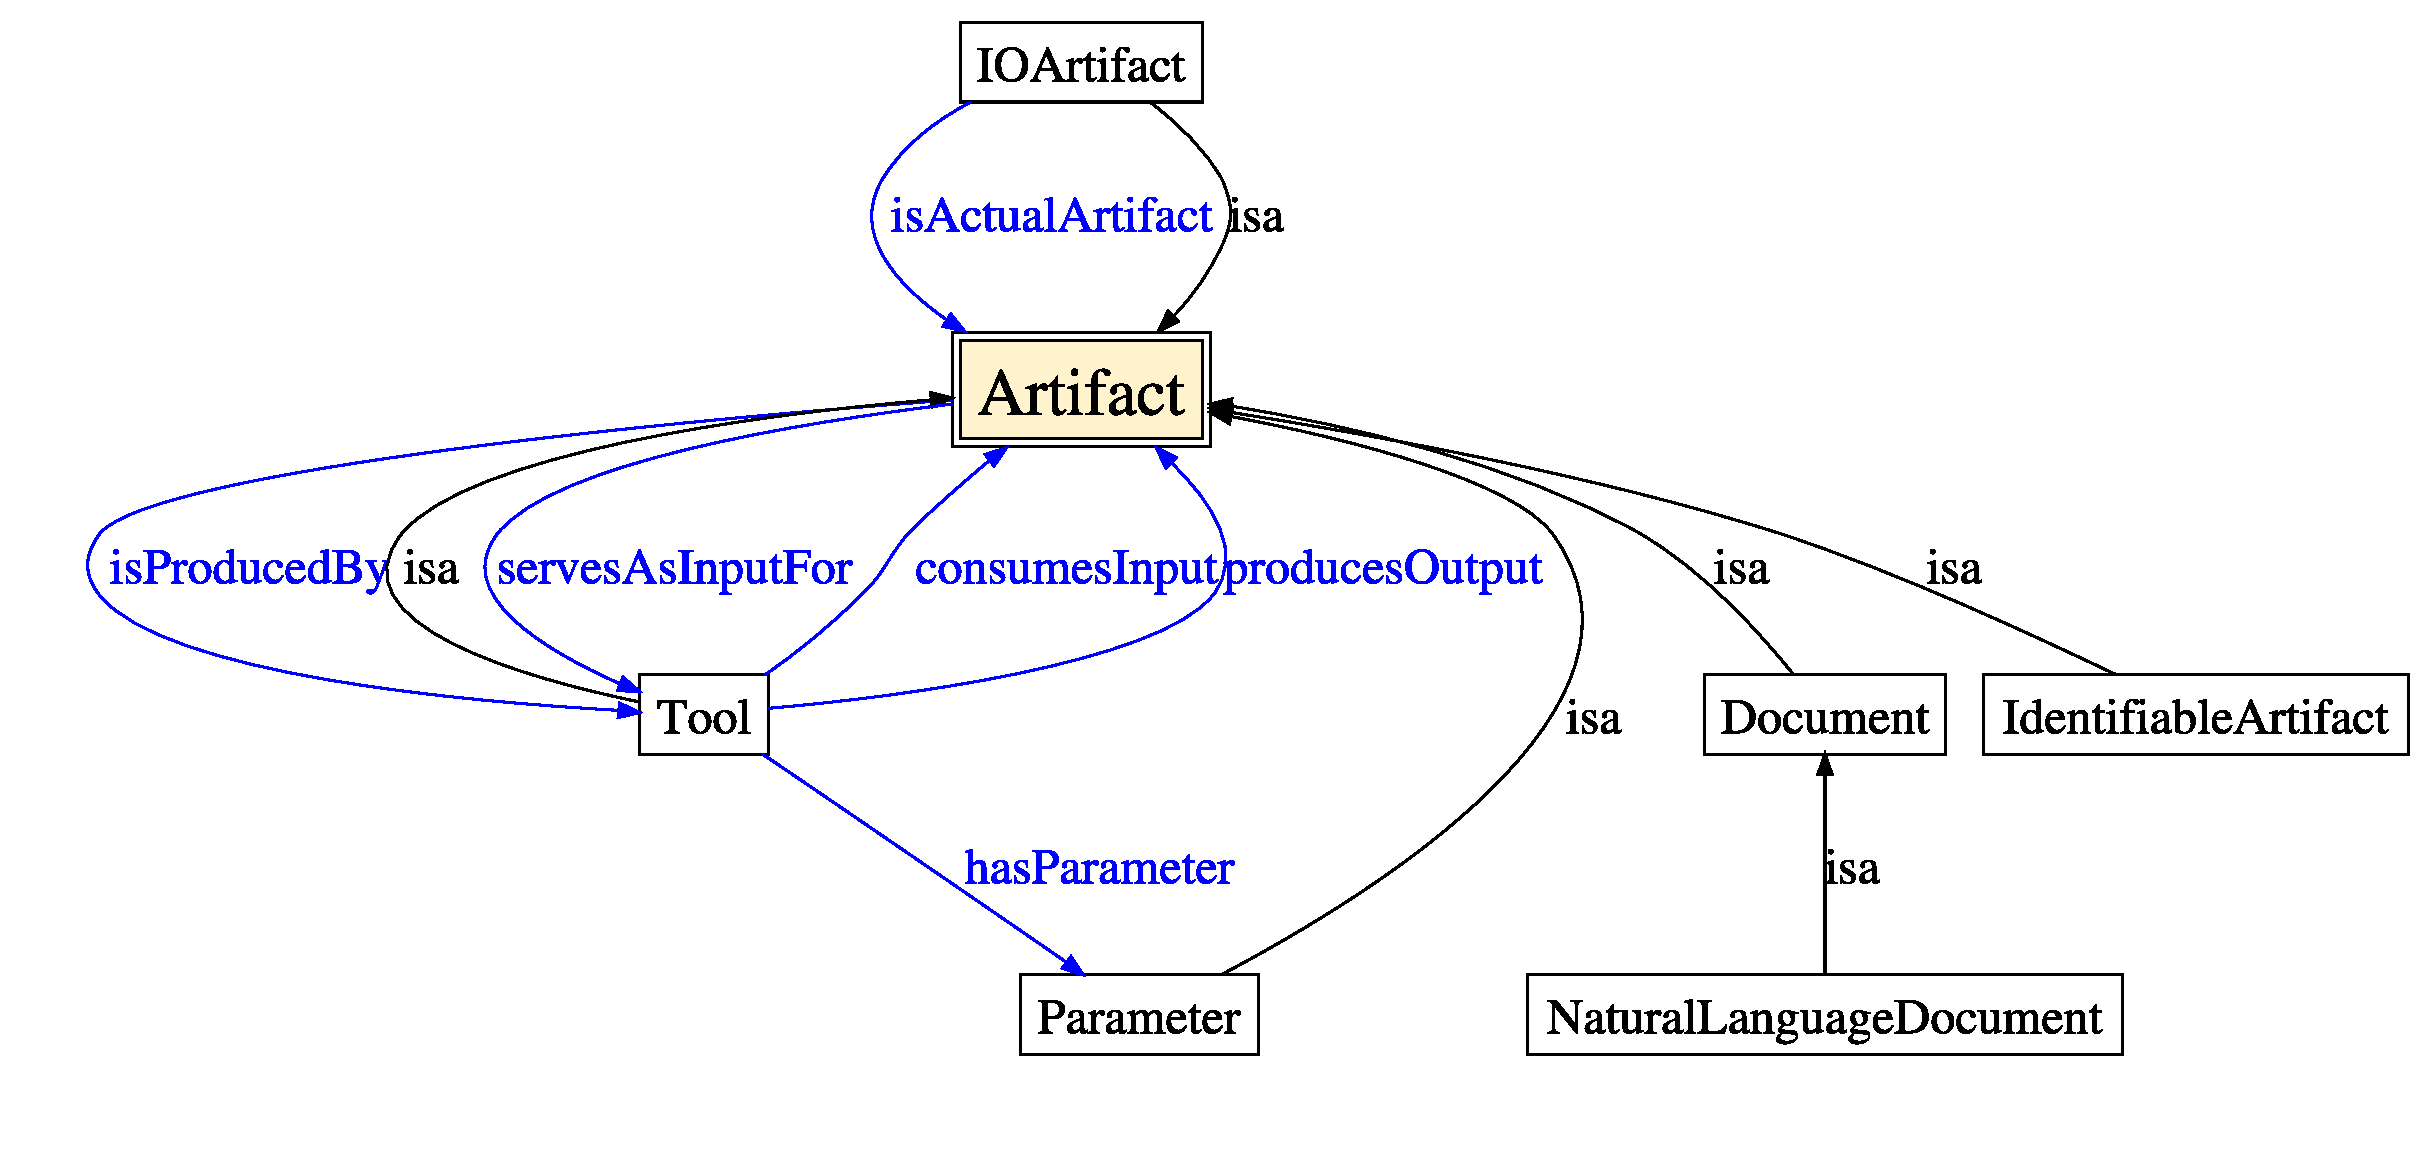
\includegraphics[width=1.0\textwidth]{pictures/artifact.pdf}
  \caption{The artifact base class with its subclasses}
  \label{fig:artifact}
\end{figure*}



We have not yet mentioned the relations \emph{servesAsInputFor} and
\emph{isProducedBy}. They are the inverse relations of
\emph{consumesInput} and \emph{producesOutput}, respectively, and have
been defined for reasons of completeness.



\begin{table}[tb]
\centering\small\sffamily
\begin{tabular}{p{0.20\textwidth}@{\hspace*{4mm}}p{0.42\textwidth}@{\hspace*{4mm}}p{0.28\textwidth}}
  \toprule 
  \textbf{Concept}&\textbf{Description} &\textbf{Example} \\
  \midrule

  Tool & Parent concept for all processing artifacts. Typically
  consumes some input and/or produces some output. & Single Document
  Summarizer, POS tagger \\

   & & \\

  Document & Artifact with a language (mandatory) & Web document,
  Java source code file \\

   & & \\

  Natural & Document with a & English Manual, \\
  Language Document & \emph{hasNaturalLanguage} property & French Novel \\

   & & \\

  Identifiable & Artifact that has some identifiable & Web document, GATE \\
  Artifact & string, e.g., a URI & processing pipeline \\

   & & \\

  Parameter & Parameter for a tool, typically with some type
  information  & Output format, desired summary length \\

   & & \\

  IOArtifact & Proxy for an input or output artifact, holding
  additional information on the relationship between the artifact and
  the consuming/producing tool  & Plain text output proxy, HTML output
  proxy \\

  \bottomrule
\end{tabular}
\caption{Sub-concepts of the \emph{Artifact} concept}
\label{tab:artifact}
\end{table}




\subsection{Specializing the Upper Ontology}
\label{sec:lsont}
The upper ontology that we have just introduced gives us several
things we need: artifacts, users, parameters, tools, etc. However, we
still lack some important NLP-specific concepts, which is why, in this
section, we substantiate the abstract upper ontology and refine it
into an ontology for language services. In particular, we include
concepts specific for the NLP subsystem in use by the \sa
architecture, GATE. Integrating a different NLP subsystem, like UIMA,
would require an alternative specialization focusing on UIMA specific
concepts and their relations.

\paragraph{New Tools and Artifacts.} We can now add a core concept for
the \sa architecture, NLP services. They are modeled as child concepts
to the \emph{Tool} concept, classifying language services in two
categories: \emph{IRTool} and \emph{NLPTool}. The semantics that we
want to convey by this separation is that an information retrieval
tool (\emph{IRTool}) finds documents, but leaves them untouched, while
an NLP tool processes documents and typically generates some new
artifact(s) from them. For NLP tools, input and output natural
languages can be specified. However, they do not have to be specified,
as there are also language-independent language services. Therefore,
if no input language is specified, we will assume that the language
service can handle any input language. Likewise, if no output language
is specified, we will assume that it can handle any output language.

Additionally to \emph{IRTool} and \emph{NLPTool}, we have one more
child concept named \emph{GATEPipeline}. While the two first concepts
imply certain semantics, the latter is defined solely via its
\emph{Format}, which has to be a certain GATE pipeline format. The
semantics of a \emph{GATEPipeline} are defined by its also being an
instance of one of the other two concepts. This means that a
\emph{GATEPipeline} can be an \emph{NLPTool} or an \emph{IRTool}.

The \emph{GATEPipeline} concept is obviously GATE specific: A sequence
of processing components is called \emph{pipeline} in GATE. In this
ontology, we do not model these processing components explicitly, as
an end user is not interested in single components of language services,
but in language services as a whole. Instances of \emph{GATEPipeline}
are the language services we offer the user through our architecture.

Having covered the \emph{Tool} extensions of our concrete ontology,
let us have a look at the artifacts they are associated with. As
mentioned, we need a semantic description of several GATE data
structures. Accordingly, we introduce new concepts as children of the
\emph{Artifact} concept. \emph{GATECorpus} represents a collection of
documents, which typically serves as input for a language service.
\emph{GATEAnnotation} instances describe the information which
language services add to a document. Annotations are organized into
annotation sets, hence we provide \emph{GATEAnnotation} with an
attribute specifying to which annotation set a given instance belongs
to. GATE annotations can have features, which are, as presented in
Section~\ref{sec:response}, included in our response
messages. Therefore, \emph{GATEAnnotation} instances can have an
unlimited number of \emph{hasFeature} attributes, which are simple
strings. \emph{GATERuntimeParameter} models parameters that control
certain aspects of a GATE pipeline, and is introduced as a sub-concept
to the already existing \emph{Parameter} concept. Along with these
artifact types, we have to introduce according new formats (remember
that artifacts are required to have a format). These are defined under
the common parent concept of \emph{GATEFormat}, which is a child of
the \emph{Format} concept.

\paragraph{Conditional Output.} The output of a tool can vary
depending on the input or on parameters: Suppose there is a language
service that produces an index of its input documents, similar to the
ones found at the back of many books.  Suppose further that this
indexer has a parameter \emph{outputFormat}, which can be set to
\emph{plain text} or \emph{html}. Therefore, the NLP service is
modelled to have two different output artifacts, a plain text file and
an HTML file. However, with the parameter settings available, only one
of them is produced at any single invocation of the NLP service, and
our server should know which one. The solution to this is provided
through the \emph{IOArtifact} concept already introduced, or, more
specifically, through a sub-concept thereof named
\emph{GATE\_OutputArtifact}.  Instances of \emph{GATE\_OutputArtifact}
have a property \emph{necessaryParameterSetting}, thus connecting an
output artifact to a certain parameter value. This parameter value is
represented through an instance of a newly introduced concept called
\emph{ParameterValuePair}. Therefore, in the example of the indexer, the
plain text output file would be associated with a
\emph{ParameterValuePair} instance holding the right parameter value
for plain text output, and the HTML output file would be associated
with one holding the value for HTML output. The server would then
compare the parameter value sent by the client to these values, and
thus know which output can actually be expected.


\paragraph{Concepts and Relationships.} The most important
additional concepts and relations of the more concrete ontology are
shown in Figure~\ref{fig:artifact2}, and also listed in
Table~\ref{tab:newconcepts}. Concepts and relations that are already
present in the upper ontology are drawn more faintly, and some of them
have been omitted entirely to keep the diagram clearer.

\begin{figure*}[tb]
  \centering
  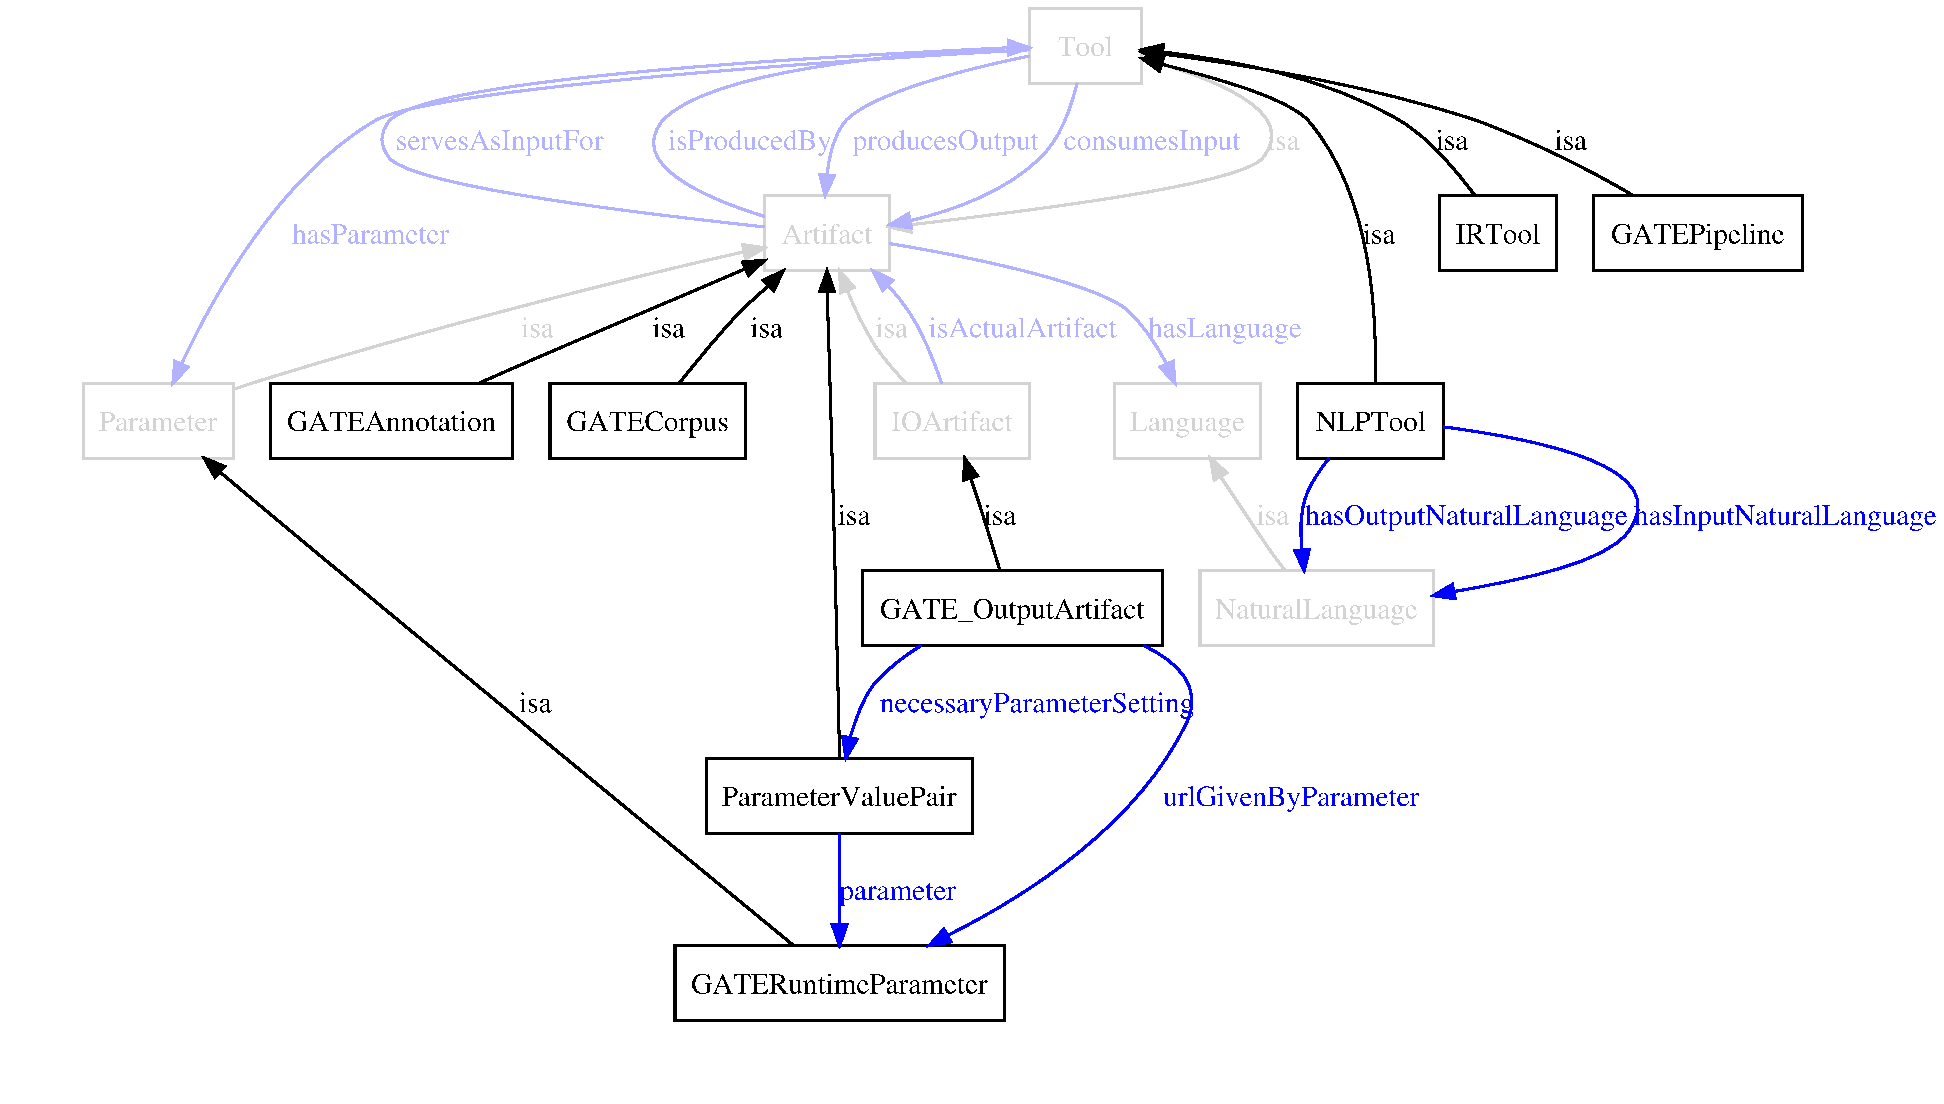
\includegraphics[width=1.0\textwidth]{pictures/artifact2.pdf}
  \caption{Additional classes introduced in the specialized ontology}
  \label{fig:artifact2}
\end{figure*}

\begin{table}[tb]
\centering\small\sffamily
\begin{tabular}{p{0.20\textwidth}@{\hspace*{4mm}}p{0.42\textwidth}@{\hspace*{4mm}}p{0.28\textwidth}}
  \toprule 
  \textbf{Concept}&\textbf{Description} &\textbf{Example} \\
  \midrule

  IRTool & Instances of this concept compile a collection of
  documents, usually in response to some query.  & \emph{YahooSearch}
  \\

   & & \\

  NLPTool & Instances of \emph{NLPTool} process or analyze documents,
  and usually produce new information from them. & \emph{Summarizer},
    \emph{Person Extractor} \\

   & & \\

  GATE Pipeline & The GATE specific implementation of a language
  service.  & \emph{Summarizer}, \emph{Person Extractor} \\

   & & \\

  GATE Annotation & GATE annotations represent linguistic and semantic
  information that has been added to a document. They can have
  \emph{hasFeature} attributes. & \emph{PersonAnnotation},
  \emph{LocationAnnotation}  \\

   & & \\

  GATE Corpus & A collection of documents, usually serving as input
  for a language service.  & \emph{StandardGATECorpus} \\

   & & \\

  GATE Runtime Parameter & Many language services accept parameters
  that influence their behaviour. Type, default value, and other
  information can be specified for a parameter.  &
  \emph{outputFileParameter}, \emph{summaryLengthParameter} \\

   & & \\

  GATE Output Artifact & Holds additional information on the
  relationship between a GATE pipeline and its possible output &
  \emph{HTMLOutputArtifact}, \emph{PlainTextOutputArtifact}  \\

   & & \\

  Parameter Value Pair & Can be used to specify certain values for a
  parameter. Usually used in combination with
  \emph{GATEOutputArtifact} and the \emph{necessaryParameterSetting}
  relation.  & \emph{htmlSetting}, \emph{plainTextSetting} \\
  \bottomrule
\end{tabular}
\caption{Concepts newly introduced in the concrete ontology for
  language services}
\label{tab:newconcepts}
\end{table}

The relation called \emph{urlGivenByParameter} connecting a GATE
output artifact to a GATE runtime parameter remains to be explained.
Often, when language services produce a file as output, they offer the
user an option to specify where this file should be stored. In our
architecture, our server has to take advantage of this so that it can
take the file and pass it on to the requesting client. The
\emph{urlGivenByParameter} relation informs the server which parameter
it can set to specify the desired output destination of an output
file.


\begin{table}[tb]
\centering\small\sffamily
\begin{tabular}{p{0.20\textwidth}@{\hspace*{2mm}}p{0.15\textwidth}@{\hspace*{2mm}}p{0.15\textwidth}@{\hspace*{2mm}}p{0.40\textwidth}}
  \toprule 
  \textbf{Property Name}&\textbf{Domain} &\textbf{Range} &\textbf{Description} \\
  \midrule

  consumesInput & Tool & Artifact & Lists the GATERuntimeParamter(s) of a language service
  \\

   & & \\

  hasFormat & Artifact & Format & Specifies the format of a language service (GATEPipeline\_Format)
  \\

   & & \\

  hasParameter & Tool & Parameter & Lists the GATERuntimeParamter of a language service
  \\

   & & \\

  producesOutput & Tool & Artifact & Specifies the output of a language service (e.g. GATEOutput\_Artifact)
  \\

   & & \\

  \bottomrule
\end{tabular}
\caption{Object Properties for Artifact}
\label{tab:art-obj-prop}
\end{table}


\begin{table}[tb]
\centering\small\sffamily
\begin{tabular}{p{0.20\textwidth}@{\hspace*{4mm}}p{0.15\textwidth}@{\hspace*{2mm}}p{0.15\textwidth}@{\hspace*{2mm}}p{0.40\textwidth}}
  \toprule 
  \textbf{Property Name}&\textbf{Domain} &\textbf{Range} &\textbf{Description} \\
  \midrule

  hasLabel & Artifact & xsd:string & Specifies the label to be shown to clients
  \\

   & & \\

  appFileName & GATEPipeline & xsd:string & The actual filename of the GATE application, without path, e.g. Durm-Indexer
  \\

   & & \\

  hasGateName & Artifact & unset & Specifies the name of the Artifact.
  \\

   & & \\

  mergeInputDocuments & Artifact & xsd:boolean & Specifies if input documents are to be merged into one before they are passed to this language service
  \\

   & & \\

  publishAsNLPService & Tool & xsd:boolean & Specifies if an NLP tool should be published to client(s)
  \\

   & & \\

  \bottomrule
\end{tabular}
\caption{Datatype Properties for Artifact}
\label{tab:art-dat-prop}
\end{table}




\begin{table}[tb]
\centering\small\sffamily
\begin{tabular}{p{0.20\textwidth}@{\hspace*{2mm}}p{0.15\textwidth}@{\hspace*{2mm}}p{0.15\textwidth}@{\hspace*{2mm}}p{0.40\textwidth}}
  \toprule 
  \textbf{Property Name}&\textbf{Domain} &\textbf{Range} &\textbf{Description} \\
  \midrule

  hasFormat & Artifact & Format & Specifies the format of a language service (Standard\_GATEAnnotation\_Format)
  \\

   & & \\  

  \bottomrule
\end{tabular}
\caption{Object Properties for GATEAnnotation}
\label{tab:ann-obj-prop}
\end{table}


\begin{table}[tb]
\centering\small\sffamily
\begin{tabular}{p{0.20\textwidth}@{\hspace*{4mm}}p{0.15\textwidth}@{\hspace*{2mm}}p{0.15\textwidth}@{\hspace*{2mm}}p{0.40\textwidth}}
  \toprule 
  \textbf{Property Name}&\textbf{Domain} &\textbf{Range} &\textbf{Description} \\
  \midrule

  hasFeature & GATEAnnotation & xsd:String & Specifies the additional features of an annotation
  \\

   & & \\

  hasGATEName & Artifact & xsd:String & The name of the Annotation
  \\

   & & \\  

  \bottomrule
\end{tabular}
\caption{Datatype Properties for GATEAnnotation}
\label{tab:ann-dat-prop}
\end{table}



\begin{table}[tb]
\centering\small\sffamily
\begin{tabular}{p{0.20\textwidth}@{\hspace*{2mm}}p{0.15\textwidth}@{\hspace*{2mm}}p{0.15\textwidth}@{\hspace*{2mm}}p{0.40\textwidth}}
  \toprule 
  \textbf{Property Name}&\textbf{Domain} &\textbf{Range} &\textbf{Description} \\
  \midrule

  hasFormat & Artifact & Format & Specifies the format of a language service (Standard\_GATEAnnotation\_Format)
  \\

   & & \\

  isActualArtifact & IOArtifact & Artifact & Specifies the actual GATEAnnotaiton Individual
  \\

   & & \\

  isProducedBy & Artifact & Tool & The Artifact that prodcues the output (e.g. GATE pipeline)
  \\

   & & \\  

  \bottomrule
\end{tabular}
\caption{Object Properties for GATEOutputArtifact}
\label{tab:out-obj-prop}
\end{table}


\begin{table}[tb]
\centering\small\sffamily
\begin{tabular}{p{0.15\textwidth}@{\hspace*{4mm}}p{0.20\textwidth}@{\hspace*{2mm}}p{0.15\textwidth}@{\hspace*{2mm}}p{0.40\textwidth}}
  \toprule 
  \textbf{Property Name}&\textbf{Domain} &\textbf{Range} &\textbf{Description} \\
  \midrule
  
  hasGATEName & Artifact & xsd:string & The name of the GATEOutputArtifact
  \\

   & & \\  

  isPerDocument & GATE\_OutputArtifact & xsd:boolean & Specifies is this artifact produced for each input document, or is it valid for a whole input corpus.
  \\

   & & \\ 
  \bottomrule
\end{tabular}
\caption{Datatype Properties for GATEOutputArtifact}
\label{tab:out-dat-prop}
\end{table}



\begin{table}[tb]
\centering\small\sffamily
\begin{tabular}{p{0.20\textwidth}@{\hspace*{2mm}}p{0.15\textwidth}@{\hspace*{2mm}}p{0.15\textwidth}@{\hspace*{2mm}}p{0.40\textwidth}}
  \toprule 
  \textbf{Property Name}&\textbf{Domain} &\textbf{Range} &\textbf{Description} \\
  \midrule

  hasFormat & Artifact & Format & Specifies the format of a language service (Standard\_GATE\_RTP\_Format)
  \\

   & & \\

  servesAsInputFor & Artifact & Tool & Specifies the tool (e.g. pipeline) that the parameter serves as input for.
  \\

   & & \\
  
  \bottomrule
\end{tabular}
\caption{Object Properties for GATERuntimeParameter}
\label{tab:run-obj-prop}
\end{table}


\begin{table}[tb]
\centering\small\sffamily
\begin{tabular}{p{0.12\textwidth}@{\hspace*{4mm}}p{0.25\textwidth}@{\hspace*{2mm}}p{0.20\textwidth}@{\hspace*{2mm}}p{0.40\textwidth}}
  \toprule 
  \textbf{Property Name}&\textbf{Domain} &\textbf{Range} &\textbf{Description} \\
  \midrule
 
  hasLabel & Artifact & xsd:string & Specifies the label to be shown to clients
  \\

   & & \\


  isOptional & IOArtifact or Parameter & xsd:boolean & Specifies if the runtime parameter for the processing resource is optional.
  \\

   & & \\ 
  
  defaultValue & GATERuntimeParameter & xsd:string & The name of the GATEOutputArtifact
  \\

   & & \\  

  hasGATEName & Artifact & xsd:string & The name of the GATERuntimeParameter
  \\

   & & \\ 

  paramType & GATERuntimeParameter & owl:oneOf\{``string'' ``double'' ``int'' ``boolean'' ``url'' ``list(string)'' ``list(double)'' ``list(int)'' ``list(boolean)'' ``list(url)''\} & Specifies The type of a parameter. Use string, double, int, or boolean for now.
  \\

   & & \\ 

  prName & GATERuntimeParameter & xsd:string & Specifies the name of the processing resource the parameter belongs to.
  \\

   & & \\ 
  \bottomrule
\end{tabular}
\caption{Datatype Properties for GATERuntimeParameter}
\label{tab:run-dat-prop}
\end{table}


We have noted that GATE pipelines contain several processing
resources, each of which can, in theory, take parameters. Obviously,
the parameter values sent by the client must be assigned correctly,
i.e., to the correct processing resources. To satisfy this
requirement, \emph{GATERuntimeParameter} instances hold an attribute
called \emph{prName}, the ``pr'' standing for ``processing
resource''. Additionally, parameters hold a \emph{paramType} and a
\emph{defaultValue} attribute.


\paragraph{Concatenation of Language Services.}
Language services can also be concatenated. In order to do this, we
introduced an attribute to the \emph{GATEPipeline} concept, called
\emph{concatenationOfPipelines}. If a language service is actually a
concatenation of several GATE pipelines. This attribute holds a
comma-separated list of the according pipeline names. We chose this
flat data type approach over object relations because it is an easier
way of guaranteeing the correct order of the language services. OWL
does not support ordering in an obvious way, and although a design
pattern for modelling sequences exists, % \cite{owlseq},
we felt that our simple approach was sufficient for the situation at
hand.


\subsubsection{Querying the \sa Ontology}
The ontology described so far now contains the information
needed to dynamically find, load, parametrize, and execute available
language services, based on user's current task and language
capabilities.  In our implementation, it is queried using Jena's
SPARQL\footnote{SPARQL Query Language for RDF, see
  \url{http://www.w3.org/TR/rdf-sparql-query/}} interface, using the
context information delivered by the client plug-in, in order to
recommend applicable Semantic Assistants.

For example, when a recommendation request is received, with a context
object saying the user knows English and German, the generated SPARQL
query should restrict the available services to those that deliver
English or German as output language. A simplified version of such a
generated query is shown below:

\begin{lstlisting}[language=SQL,xleftmargin=8mm,columns=flexible]
SELECT ?x ?name
WHERE { ?x sa:hasGATEName ?name  .
         {?x cu:hasFormat sa:GATECorpusPipeline_Format}  . {
             {?x sa:hasOutputNaturalLanguage cu:en}  UNION 
                 {?x sa:hasOutputNaturalLanguage cu:de}}
}
\end{lstlisting}
Once the SPARQL query has been generated, it is passed to the
\texttt{OntModel} instance containing the language service
descriptions. The results are then retrieved from this object,
converted into the corresponding client-side versions, and returned to
the client.

For additional information on the communication between the SA server,
CSAL, and clients, please refer to Chapter~\ref{chap:dev}.